\chapter{Modelling}
The task of reconstructing an unknown surface from a point cloud is not a trivial task. Especially not when this point cloud is obtained through a camera mounted as the tool on a robot arm. To be able to reconstruct the full surface several views of the object are required, which mean that several point clouds are required to be aligned with each other and stitched together. The modelling component of this system is divided into two sub-components, the first component described in this chapter is filtering and the second component described is the reconstruction component. 

\section{Filtering}
Filtering of raw point clouds is required because of several different reasons. The number of points delivered to the modelling component from the raw point clouds is huge, so filtering non-interesting points away creating a region-of-interest (ROI) in the raw point clouds. Lowering the number points in each cloud delivered to the modelling component is required such the workload can be kept within an acceptable range. The number of points can be further reduced by down-sampling the points left in the ROI by the cut-off filter. A voxel-grid filter utilised for down-sampling also creates the advantage of equal sampling density, but the disadvantage is that the down-sampling means loss of information, and therefore there is a trade off between speed and level of detail of the reconstruction process.  

\begin{figure}[htb]
	\begin{center}
		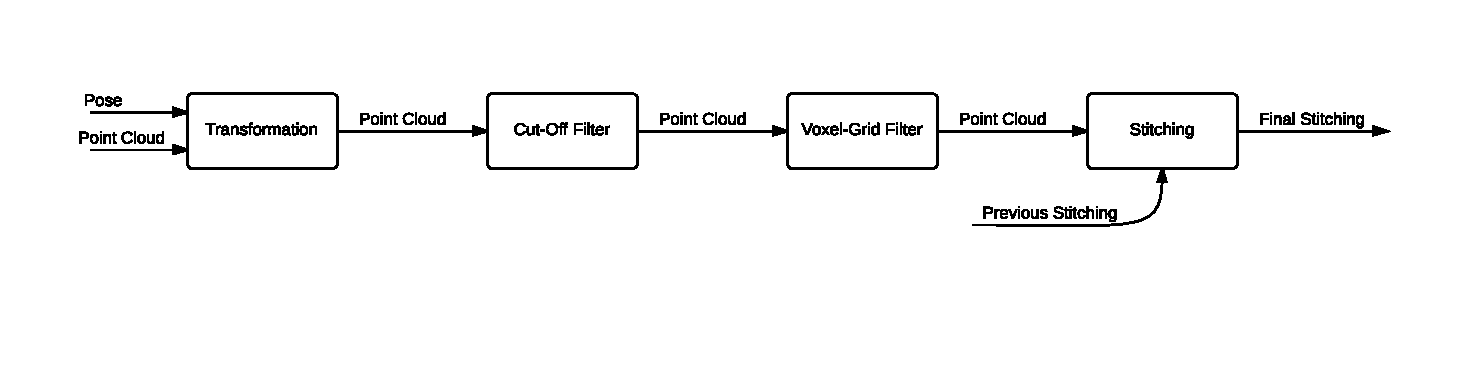
\includegraphics[scale=0.6,trim=20 70 0 20]{graphics/07_modelling/FilterFlow.pdf}%trim=l b r t
		\caption{Illustrates the flow through the filter.}
		\label{fig:filter_flow}
	\end{center}
\end{figure}

In figure \ref{fig:filter_flow} an illustration of the flow through the filter can be seen. The vision layer is delivering a point cloud for each individual view, along with this point cloud a pose of the frame in which the points are recorded is delivered. These two sets of data is delivered to the ROS node which handles filtering, this node filters each individual cloud and stitches each of them together in a common cloud. This common cloud, when finished, is sent to the reconstruction layer. In the sections below is a brief description of the components shown in figure \ref{fig:filter_flow}. 

\subsection{Point cloud library}
The Point Cloud Library (PCL) utilised in this project is a library which provide functionality for working on 3D point clouds. PCL delivers a variety of functionality such as filters, segmentation, surface reconstruction, kd- and oc-trees, visualisation, etc. PCL can be found at http://www.pointclouds.org/, along with documentation and tutorials.

\subsection{Point cloud transformation}
Messages received from the vision layer needs to be processed before filtering. This is because the messages delivered to the modelling component contain a point cloud and a pose of the current camera view. The coordinates of the individual points in the cloud are related to the camera frame, but this frame is moving around the object so a transformation of points is needed such they can be related a common static frame.

\begin{figure}[htb]
	\begin{center}
		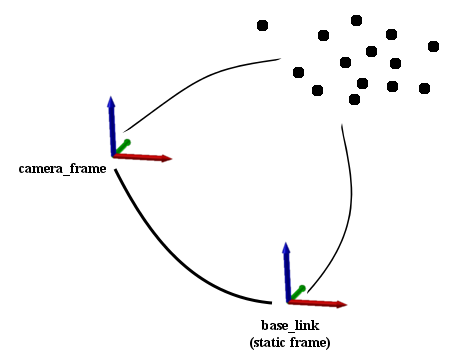
\includegraphics[scale=0.7,trim=0 0 0 0]{graphics/07_modelling/pctransform.png}%trim=l b r t
		\caption{Illustrates points in different frames.}
		\label{fig:filtering_transform}
	\end{center}
\end{figure}

\subsection{Cut-off filter}
The cut-off filter utilised is the implementation from PCL, \texttt{pcl::PassThrough< \ldots >}. A cut-off filter is utilised to create a ROI in the transformed point cloud, partly because the number of points needs to be reduced with respect to processing time and then because the region in which the object resides is fairly small to the region which is recorded by the camera.

\subsection{Voxel-grid filter}
The voxel-grid down-samples the left overs from the cut-off filtering. The down-sampling causes loss of information which mean that surface details are lost in the process, so the amount of down-sampling should be chosen with respect to processing time versus level of detail to be reconstructed. The PCL library luckily have such functionality (\texttt{pcl::VoxelGrid< \ldots >}) which is utilised in the filtering sub-component.\\
\\
The voxel-grid filter works by splitting down the ROI into smaller regions (voxels) of certain resolution in which each of the voxels are analysed. Figure \ref{fig:filtering_voxel_grid} show the principle of the voxel-grid. A new point is approximated for each voxel, the new point is approximated by the points centroid which is contained in the voxel. This method is a little slower compared to just placing the new point in the center of the voxel, but it helps save some more detailed information about the surface curvature.
\begin{figure}[htb]
	\begin{center}
		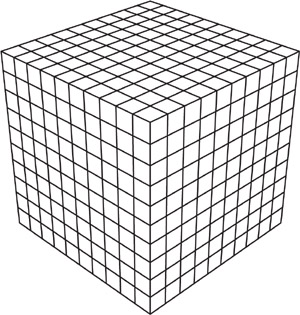
\includegraphics[scale=0.7,trim=0 0 0 0]{graphics/07_modelling/cube.jpg}%trim=l b r t
		\caption{Illustrates a cube consisting of 10x10x10 cubes which resembles the voxel-grid filter.}
		\label{fig:filtering_voxel_grid}
	\end{center}
\end{figure}

\subsection{Point cloud stitching}
\marginnote{Subsection not finished}

The individual point clouds from the individual views of the object are passed through the filter, the individual cloud is then stitched into another common cloud which is assembled from a number of individual clouds, predetermined by the decision making layer. The stitching of each cloud happens in the static frame, due to the transformation of the input to the filter node. The point clouds are stitched in the order at which they are received, thus the first frame becomes a sort of reference frame for the following frames. This is because the algorithm used for stitching the clouds together actually calculates a transform at which new incoming point clouds are transformed. The algorithm utilised for stitching is Iterative Closest Point (ICP). This is also implemented in in PCL and therefore this implementation (\texttt{pcl::IterativeClosestPointNonLinear< \ldots , \ldots >}) of the algorithm utilised. The ICP algorithm has it downsides. For example if a cloud is not aligned correctly, this will cause an error to propagate thought to the following clouds which could lead to a rather distorted model of the object of interest\cite{choe2007registration}. The algorithm will be described in further details in chapter \texttt{ref??}\marginnote{Ref til calibration chapter}.
\section{Surface reconstruction}
Surface reconstruction from a large set of unstructured points obtained through laser scanning techniques or stereopsis is not a trivial task but nonetheless it is useful in many applications. For example a surface reconstruction could aid a robots end effector grasping some unknown object \cite{Wang2005}. Many methods for surface reconstruction exist in different domains of science, some algorithms are based on neural network approaches  \cite{Wu2007}, others are based on sculpting or region growing algorithms (e.g \cite{Bernardini1999} and \cite{Amenta2001}) used in computational geometry, some utilise an implicit method framework to represent incoming data as a surface \cite{Kazhdan2006} and \cite{Dong2011}.\\
\\
In 1999 F. Bernardini \textit{et al}. proposed in a fairly simple algorithm (Ball Pivoting Algorithm (BPA)) for reconstruction of surfaces from point clouds sampled over smooth objects \cite{Bernardini1999}. BPA is pivoting a sphere of a certain diameter around an edge of a seed triangle. Pivoting the sphere around all the edges is connecting three points to form a new triangle and so on. BPA is a part of the region growing algorithms as this algorithm uses a seed triangle builds the surface around this and outward. The algorithm is fairly easy to work with as it has one parameter which decides the radius of the sphere and that is it. N. Amenta \textit{et al}. proposed in 2001 \cite{Amenta2001} the power crust algorithm, which essentially is a three dimensional Voronoi approach \cite{Ledoux2007}. The power crust algorithm is well defined and proven which makes it one of the most known algorithm regarding surface reconstruction. This algorithm is a sculpting algorithm in computational geometry. Common for those algorithms mentioned is that these are explicit methods which requires neighboring information which leads to high computational time consumption. Therefore methods mentioned above are not well suited for reconstruction of large data sets.\\
\\
In 2006, M. Kazhdan \textit{et al}. proposed in \cite{Kazhdan2006} an algorithm which resides in the implicit method framework, this algorithm is called Poisson Surface Reconstruction (PSR). PSR is a fitting scheme that allow solving for the indicator function of the surface. It is shown in \cite{Kazhdan2006} this approach of fitting a surface resembles the Fast Fourier Transform (FFT). In \cite{Kazhdan2006} it is shown that the FFT approach requires five times as much space but is approximately double as fast while creating approximately the same number of triangles. The real advantage of the Poisson approach is that it is scalable and therefore does not rely on a uniform distribution of points and thus a higher degree of details can be reconstructed in areas where the point density is higher.\\
J. Manson \textit{et al}. did in 2008 propose a wavelet approach of the problem of reconstructing surfaces of large sets of unstructured points \cite{Manson2008}. The method is robust to noise in data because it is relying on implicit methods as PSR, and is therefore well-suited for reconstruction of real data which is overlayed with some random noise. The wavelet approach an advantages over PSR, the wavelet approach is able to reconstruct non-closed surfaces in opposition to PSR \cite{Kazhdan2006}. Using the Haar wavelet synthesise an acceptable surface if the points are well-aligned, else more smooth wavelets can be used such as Daubechies-2. Using octrees and small-support wavelets makes the synthesisation very fast, smaller support equals less computational time and space. Using Daubechies-2 compared to Haar increases computational time by a scale of four, and the space consumption is upscale by approximately four as well. As the methods for reconstruction mentioned first does not guarantee watertight mesh and does not work very well with large point sets, mean those methods are not of interest for further studies. The PSR and the wavelet approach both does estimate an indicator function of the surface, but each handles this indicator function differently. As these method is based on implicit methods they are more robust to noise in the input and approximates the surfaces better compared to the methods mentioned first.

\subsection{Overview of reconstruction scheme}
The wavelet method for surface reconstruction chosen for this custom implementation is highly inspired by the description in \cite{Manson2008}. One main reason for using wavelets for the analysis of the surface compared to more conventional methods like FFT is that wavelets support localisation in spatial and frequency(scale) domains. This mean that analysis is made locally instead of globally, which leads to the possibility of reconstructing finer details in input data, that would otherwise be hidden by the global analysis. PSR is approximating an indicator function\marginnote{ref: indicator function} of the surface by solving a Poisson equation\marginnote{ref: Poisson eq.}. In the wavelet approach an indicator function is also estimated, but the way it is done is different. The wavelet approach approximates the wavelet coefficients of the indicator function by making a multi resolution analysis (MRA) of the input data\marginnote{ref: MRA, coeffs}. After the coefficients have been calculated ...

\subsection{Indicator function}
The method mentioned in \cite{Manson2008} defines the indicator function of the surface $\partial M$ of an object $M$ to be as follows

\begin{equation}
	\chi_M(\textbf{x}) =  
	\label{eq:indicator_fnc}
\end{equation}



\begin{equation}
	c^e_{j,\textbf{k}} \approx 2^{3j \over 2} \sum_{p_i \in \partial M \cap \textit{supp}(\psi^e_{j,\textbf{k}})} \vec{F}^e_{j,\textbf{k}} (p_i) \cdot \vec{n}_i d \sigma_i 
	\label{eq:wavelet_coeffs}
\end{equation}

\subsection{Mesh generation}

\subsection{Implementation}
The surface reconstruction is implemented in ROS node making it compatible with the rest of the system. The assembled point cloud is passed from the filter node to the reconstruction node. PCL is used for estimating normals of the points in the assembled point cloud. 

\subsection{Results}